%% Algoritmi

\subsection{Filtraggio software}
\label{ssez:filtraggio}

Prima di iniziare qualsiasi elaborazione dei dati acquisiti
occorre eseguire delle operazioni di filtraggio,
necessarie a ridurre il rumore e
a diminuire le dimensioni.

Il filtro passabasso per ridurre il rumore è
una media mobile di lunghezza 13;
determinata empiricamente.
Si esegue poi un sottocampionamento di un fattore 5.





\subsection{Classificazione}
\label{ssez:classificazione}

Saranno esposte in seguito i concetti fondamentali
della teoria dei \textit{cluster}
(il termine proposto da \cite{cit:fuzzy} è \textit{botriologia}\footnotemark{}),
e le principali tecniche di classificazione
fino alle macchine a vettori di supporto (\ac{svm}).


\subsubsection{Estrazione delle caratteristiche}
\label{sssez:estrazione}

Al fine di ridurre il più possibile lo sforzo computazionale,
\textbf{aumentando al contempo il significato delle variabili,}
occorre cercare le caratteristiche più rappresentative
dei movimenti in questione.
Tali caratteristiche sono funzione dei movimenti analizzati,
degli esempi proposti e
della classificazione cercata;
possono essere proprietà statistiche come media e varianza,
relazioni più complesse nello spazio e nel tempo
o semplici limitazioni (troppo ampio, troppo lento...).

Queste osservazioni assumono tra l'altro che i dati
siano già in formato vettoriale,
che abbiano quindi la forma di sequenze di numeri
messi in fila o in tabelle di qualsivoglia dimensione.
Se così non fosse, l'estrazione delle caratteristiche
non sarebbe soltanto una comodità per ridurre la mole di calcoli
bensì una necessità per portare gli oggetti in esame
in uno spazio dove queste elaborazioni siano possibili.
Si ritornerà sull'argomento trattando
la mappatura delle \ac{svm}.


\subsubsection{Scelta delle caratteristiche}
\label{sssez:scelta}

Un approccio al problema, tipico della logica sfumata,
\`e conoscere a priori il gesto da valutare e
implementare manualmente le regole di classificazione nel codice della macchina.
Si ottiene così una soluzione specifica.

Quando si vuole invece scoprire queste regole,
occorre avanzare delle ipotesi e poi vagliarle.
Se non si conoscono a priori le caratteristiche significative,
si può procedere estraendone in sovrannumero e
calcolando a posteriori quelle più importanti.
Fatto questo, si possono ``scartare'' le discriminazioni evidenti
e scegliere di concentrarsi sugli aspetti più sottili.
Si preferisce questa soluzione per la sua generalità.






\subsection{Tecniche di classificazione}
Panoramica sulle tecniche statistiche e di apprendimento automatico utili al problema della classificazione.

\subsubsection{K-mean clustering}
Tecnica di classificazione non supervisionata
(non bisogna etichettare i dati prima di far partire l'algoritmo)
che consiste in
\begin{enumerate}
  \item{gettare pi\`u o meno casualmente \emph{K centroidi} nello spazio}
  \item{etichettare ogni punto con l'ID del centroide pi\`u vicino}
  \item{spostare ogni centroide sulla media dei punti a esso assegnati}
  \item{ripetere dal punto 2 finch\'e i centroidi non sono quasi fermi}
\end{enumerate}

\paragraph{Con Matlab}
Il toolbox $statistics$ mette a disposizione il comando $kmeans$ che,
ricevendo in ingresso i punti e il numero di gruppi desiderati,
restituisce le etichette per ogni punto e le coordinate dei centroidi.
Altro scalaggio per visualizzare i dati in 2D.

\paragraph{Crossvalidazione}
Il numero di centri $K$ \`e fissato a priori
ma non sempre si hanno buoni motivi per scegliere un valore pittosto che un altro.
Per trovare il $K$ migliore si fa di solito correre l'algoritmo pi\`u volte,
ogni volta cambiando il $K$ e valutando le prestazioni.
L'insieme dei dati dev'essere preventivamente diviso
in un gruppo di addestramento e un gruppo di test, o validazione.



\subsubsection{Il percettrone classico}
Il percettrone cerca di dividere in due l'universo
mettendoci in mezzo un piano.
Tale piano \`e individuato dai pesi del neurone
e da una soglia, che in pratica \`e un ulteriore sinapsi
con l'ingresso sempre a 1 (o -1, se si preferisce).
La funzione di attivazione può essere la funzione segno, visto che c'è un solo neurone. Se invece si utilizza una rete neurale a più strati con \textit{backpropagation}, occorre adoperare esponenziali o tangenti iperboliche
(\textsc{Equazione~\ref{eq:perceptron}}).

Per ogni vettore d'ingresso
il percettrone calcola 
\begin{equation}
	y = sgn \left(x \cdot w - \theta \right);
	\label{eq:perceptron}
\end{equation}
in fase di addestramento, si confronta l'uscita calcolata
con quella desiderata: $e=d-y$
e si correggono i pesi di un fattore $\Delta w = a\,e\,x$,
dove $a \in [0, 1]$ \`e il fattore di apprendimento.
Analogo per la soglia.

Ad apprendimento concluso i pesi non variano pi\`u
ed il piano di separazione \`e finalmente individuato
dall'equazione \ref{eq:perceptron}, posta uguale a 0.

Una rappresentazione grafica di classificazione eseguita da un percettrone è illustrata in \textsc{Figura~\ref{fig:clus_perc}}

\begin{figure}
\centering
\begin{tikzpicture}

% \draw [red] (-3,-3) grid (3,3);
\draw (-1,1) circle (.25);
\draw (-1,-1) circle (.25);
\draw (-2,-1) circle (.25);
\draw (-2,-2) circle (.25);
\draw (-3,1) circle (.25);

\draw (1,1) ++(-.2,-.2) rectangle ++(.4,.4);
\draw (1,-1) ++(-.2,-.2) rectangle ++(.4,.4);
\draw (2,-1) ++(-.2,-.2) rectangle ++(.4,.4);
\draw (2,-2) ++(-.2,-.2) rectangle ++(.4,.4);
\draw (3,1) ++(-.2,-.2) rectangle ++(.4,.4);

% \node [fill] at (3,3) {};
\draw (-1,-3) -- (1,3)
 node[pos=.7,sloped,above]{iperpiano di separazione};
% % \draw (0,-3) -- (0,3)
% %  node[pos=.8,sloped]{perceptron};


\end{tikzpicture}
\caption{Classificazione con il percettrone}
\label{fig:clus_perc}
\end{figure}

\begin{figure}
\centering
 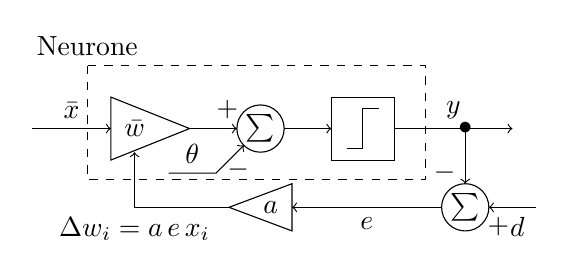
\begin{tikzpicture}
%
%% Ingresso
  \draw[->](0,0)--(1,0)
    node[pos=.5,above]{\(\bar{x}\)};
%
%% Cornice del neurone
  \draw [dashed, line join=round] (.7,.8) rectangle (5,-.65)
    node [pos=0, above] {Neurone};
%
%% Blocchi del neurone
  \draw (1,-.4)--(2,0)--(1,.4)--cycle;
  \node (w) at (1.3,0) {\(\bar{w}\)};
  \draw[->](2,0)-- ++(.6,0)
    node[pos=.8,above]{\(+\)};
  \draw[<-](2.9,0) ++(-135:.3)--
    ++(-135:.5) node[pos=.2,below]{$-$}
    -- ++(-.6,0)
    node[pos=.5,above]{$\theta$};
  \draw	(2.9,0) node{\(\sum\)} circle (.3);
  \draw[->](3.2,0)-- ++(.6,0);
  \draw (3.8,.4) rectangle ++(.8,-.8);
  \draw (4,-.25)-|(4.2,0)|-(4.4,.25);
%
%% Uscita
  \draw[->](4.6,0)-- ++(1.5,0)
    node[pos=.5,above]{\(y\)};
%
%% Retroazione
  \draw[->](5.5,0)-- ++(0,-.7)
    node[pos=0]{\(\bullet\)}
    node[pos=.8,left]{$-$};
  \draw	(5.5,-1) node{$\sum$} circle (.3);
  \draw[<-](5.8,-1)-- ++(.6,0)
    node[pos=0.2,below]{$+$}
    node[pos=0.6,below]{$d$};
  \draw[<-](1.3,-.3) |- (2.5,-1)
    node[pos=.5,,below]{\(\Delta w_i = a\,e\,x_i\)};
  \draw (3.3,-.7)--(2.5,-1)--(3.3,-1.3)--cycle;
  \node (a) at (3.03,-1) {$a$};
  \draw[<-](3.3,-1)--(5.2,-1)
    node[pos=.5,below]{$e$};
    
\end{tikzpicture}

 \caption{Schema a blocchi del percettrone}
 \label{fig:perceprton}
\end{figure}

\subsubsection{L'apprendimento competitivo}
Apparentemente simile al K~-~means,
\`e l'apprendimento competitivo\footnotemark{}.

\footnotetext{\,Non sono la stessa cosa e non portano agli stessi risultati}

Consiste nello strutturare una rete di $K$ neuroni
ciascuno con il suo vettore dei pesi
inizialmente casuale ma sempre di modulo 1.
In questo modo a ogni neurone \`e assegnato un versore
in un qualche spazio.
I neuroni sono tra loro collegati tramite linee di segnali inibitori.
Quando le coordinate di un punto di addestramento
sono date in pasto alla rete,
ci sar\`a un neurone che indica in quella direzione,
o per lo meno un neurone sar\`a pi\`u vicino degli altri:
questo \`e l'unico neurone autorizzato ad apprendere
e modificher\`a i suoi pesi in maniera da avvicinarsi
un po' alla direzione del punto.
L'apprendimento degli altri neuroni \`e inibito.

Questa tecnica richiede ulteriori pretrattamenti dei dati in ingresso
in maniera che siano distribuiti (meglio possibile)
su una sfera centrata nell'origine.